\documentclass[12pt]{beamer}
\usepackage{../Estilos/BeamerFC}
\usepackage{../Estilos/ColoresLatex}
\usepackage{courier}
\usepackage{listingsutf8}
\usepackage{listings}
\usepackage{xcolor}
\usepackage{textcomp}
\usepackage{color}
\definecolor{deepblue}{rgb}{0,0,0.5}
\definecolor{brown}{rgb}{0.59, 0.29, 0.0}
\definecolor{OliveGreen}{rgb}{0,0.25,0}
% \usepackage{minted}

\DeclareCaptionFont{white}{\color{white}}
\DeclareCaptionFormat{listing}{\colorbox{gray}{\parbox{0.98\textwidth}{#1#2#3}}}
\captionsetup[lstlisting]{format=listing,labelfont=white,textfont=white}
\renewcommand{\lstlistingname}{Código}


\definecolor{Code}{rgb}{0,0,0}
\definecolor{Keywords}{rgb}{255,0,0}
\definecolor{Strings}{rgb}{255,0,255}
\definecolor{Comments}{rgb}{0,0,255}
\definecolor{Numbers}{rgb}{255,128,0}

\makeatletter

\newif\iffirstchar\firstchartrue
\newif\ifstartedbyadigit
\newif\ifprecededbyequalsign

\newcommand\processletter
{%
  \ifnum\lst@mode=\lst@Pmode%
    \iffirstchar%
        \global\startedbyadigitfalse%
      \fi
      \global\firstcharfalse%
    \fi
}

\newcommand\processdigit
{%
  \ifnum\lst@mode=\lst@Pmode%
      \iffirstchar%
        \global\startedbyadigittrue%
      \fi
      \global\firstcharfalse%
  \fi
}

\lst@AddToHook{OutputOther}%
{%
  \lst@IfLastOtherOneOf{=}
    {\global\precededbyequalsigntrue}
    {}%
}

\lst@AddToHook{Output}%
{%
  \ifprecededbyequalsign%
      \ifstartedbyadigit%
        \def\lst@thestyle{\color{orange}}%
      \fi
    \fi
  \global\firstchartrue%
  \global\startedbyadigitfalse%
  \global\precededbyequalsignfalse%
}

\lstset{ 
language=Python,                % choose the language of the code
basicstyle=\footnotesize\ttfamily,       % the size of the fonts that are used for the code
numbers=left,                   % where to put the line-numbers
numberstyle=\scriptsize,      % the size of the fonts that are used for the line-numbers
stepnumber=1,                   % the step between two line-numbers. If it is 1 each line will be numbered
numbersep=5pt,                  % how far the line-numbers are from the code
backgroundcolor=\color{white},  % choose the background color. You must add \usepackage{color}
showspaces=false,               % show spaces adding particular underscores
showstringspaces=false,         % underline spaces within strings
showtabs=false,                 % show tabs within strings adding particular underscores
frame=single,   		% adds a frame around the code
tabsize=2,  		% sets default tabsize to 2 spaces
captionpos=t,   		% sets the caption-position to bottom
breaklines=true,    	% sets automatic line breaking
breakatwhitespace=false,    % sets if automatic breaks should only happen at whitespace
escapeinside={| |},  % if you want to add a comment within your code
stringstyle =\color{OliveGreen},
otherkeywords={as, np.array, np.concatenate, np.linspace, linspace, interpolate.interp1d, kind, plt.plot, .copy, np.arange, np.cos, np.pi, lw, ls, label, splrep, splev, plt.legend, loc, plt.title, plt.ylim, plt.show, sign, math.ceil, math.log, np.sqrt, np.exp, np.zeros, plt.xlabel, plt.ylabel, plt.xlim, np.identity, random, np.dot, np.outer, np.diagonal },             % Add keywords here
keywordstyle = \color{blue},
commentstyle = \color{darkcerulean},
identifierstyle = \color{black},
literate=%
         {á}{{\'a}}1
         {é}{{\'e}}1
         {í}{{\'i}}1
         {ó}{{\'o}}1
         {ú}{{\'u}}1
%
%keywordstyle=\ttb\color{deepblue}
%fancyvrb = true,
}

\lstdefinestyle{FormattedNumber}{%
    literate={0}{{\textcolor{red}{0}}}{1}%
             {1}{{\textcolor{red}{1}}}{1}%
             {2}{{\textcolor{red}{2}}}{1}%
             {3}{{\textcolor{red}{3}}}{1}%
             {4}{{\textcolor{red}{4}}}{1}%
             {5}{{\textcolor{red}{5}}}{1}%
             {6}{{\textcolor{red}{6}}}{1}%
             {7}{{\textcolor{red}{7}}}{1}%
             {8}{{\textcolor{red}{8}}}{1}%
             {9}{{\textcolor{red}{9}}}{1}%
             {.0}{{\textcolor{red}{.0}}}{2}% Following is to ensure that only periods
             {.1}{{\textcolor{red}{.1}}}{2}% followed by a digit are changed.
             {.2}{{\textcolor{red}{.2}}}{2}%
             {.3}{{\textcolor{red}{.3}}}{2}%
             {.4}{{\textcolor{red}{.4}}}{2}%
             {.5}{{\textcolor{red}{.5}}}{2}%
             {.6}{{\textcolor{red}{.6}}}{2}%
             {.7}{{\textcolor{red}{.7}}}{2}%
             {.8}{{\textcolor{red}{.8}}}{2}%
             {.9}{{\textcolor{red}{.9}}}{2}%
             {\ }{{ }}{1}% handle the space
         ,%
          %mathescape=true
          escapeinside={__}
          }



\usetheme{Dresden}
\usecolortheme{seahorse}
%\useoutertheme{default}
\setbeamercovered{invisible}
% or whatever (possibly just delete it)
\setbeamertemplate{section in toc}[sections numbered]
\setbeamertemplate{subsection in toc}[subsections numbered]
\setbeamertemplate{subsection in toc}{\leavevmode\leftskip=3.2em\rlap{\hskip-2em\inserttocsectionnumber.\inserttocsubsectionnumber}\inserttocsubsection\par}
\setbeamercolor{section in toc}{fg=blue}
\setbeamercolor{subsection in toc}{fg=blue}
\setbeamercolor{frametitle}{fg=blue}
\setbeamertemplate{caption}[numbered]

\setbeamertemplate{footline}
\beamertemplatenavigationsymbolsempty
\setbeamertemplate{headline}{}

\makeatletter
\setbeamercolor{section in foot}{bg=gray!30, fg=black!90!orange}
\setbeamercolor{subsection in foot}{bg=blue!30!yellow, fg=red}
\setbeamertemplate{footline}
{
  \leavevmode%
  \hbox{%
  \begin{beamercolorbox}[wd=.333333\paperwidth,ht=2.25ex,dp=1ex,center]{section in foot}%
    \usebeamerfont{section in foot} \insertsection
  \end{beamercolorbox}}%
  \begin{beamercolorbox}[wd=.333333\paperwidth,ht=2.25ex,dp=1ex,center]{subsection in foot}%
    \usebeamerfont{subsection in foot}  \insertsubsection
  \end{beamercolorbox}%
  \begin{beamercolorbox}[wd=.333333\paperwidth,ht=2.25ex,dp=1ex,right]{date in head/foot}%
    \usebeamerfont{date in head/foot} \insertshortdate{} \hspace*{2em}
    \insertframenumber{} / \inserttotalframenumber \hspace*{2ex} 
  \end{beamercolorbox}}%
  \vskip0pt%
\makeatother 

\makeatletter
\patchcmd{\beamer@sectionintoc}{\vskip1.5em}{\vskip0.8em}{}{}
\makeatother

\usefonttheme{serif}

\title{\large{Cálculo de raíces}}
\subtitle{Tema 2 - Operaciones matemáticas básicas}
\author{M. en C. Gustavo Contreras Mayén}
\date{}

\begin{document}
\maketitle

\section*{Contenido}
\frame{\tableofcontents[currentsection, hideallsubsections]}

\section{Bases generales}
\frame{\tableofcontents[currentsection, hideothersubsections]}
\subsection{Cálculo de raíces}

\begin{frame}
\frametitle{Cálculo de raíces}
Sea $y = f (x)$.  
\\
\bigskip
Los valores de $x$ que hacen que $y = 0$ se denominan \textcolor{blue}{raíces de la ecuación}.
\end{frame}
\begin{frame}
\frametitle{Cálculo de raíces}
El teorema fundamental del álgebra indica que todo polinomio de grado $n$, tiene $n$ raíces.
\\
\bigskip
\pause
En el caso de las raíces reales, corresponden a los valores de $x$ que hacen que la función corte el eje de las abscisas:
\end{frame}
\begin{frame}
\frametitle{Ejemplo de la función seno (x)}
\begin{figure}
	\centering
	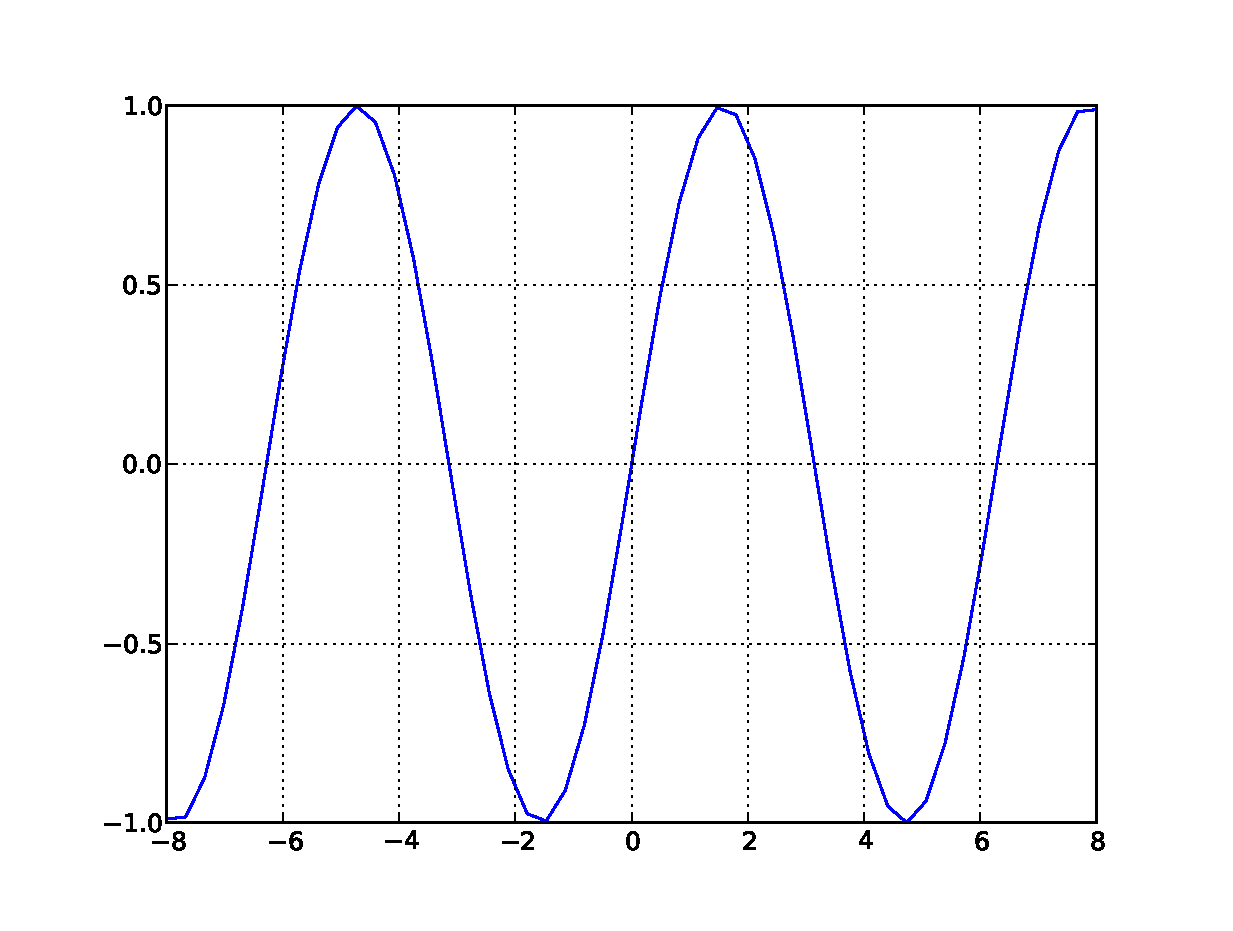
\includegraphics[scale=0.4]{Imagenes/raices00.eps}
	\caption{La función tiene varias raíces en el intervalo.} 
\end{figure}
\end{frame}
\begin{frame}
\frametitle{Tipo de raíces}
Las raíces de un polinomio pueden ser reales o complejas.
\\
\bigskip
\pause
Si un polinomio tiene coeficientes reales:
\begin{align*}
a_{0}, a_{1}, a_{2}, \ldots, a_{n-1}, a_{n}
\end{align*}
entonces todas las raíces complejas siempre ocurrirán en pares conjugados complejos.
\end{frame}
\begin{frame}
\frametitle{Tipo de raíces}
Por ejemplo, un polinomio cúbico tiene la siguiente forma general:
\pause
\begin{align*}
f (x) = a_{0} \: x^{3} + a_{1} \: x^{2} + a_{2} \: x + a_{3}
\end{align*}
\setbeamercolor{item projected}{bg=aqua,fg=black}
\setbeamertemplate{enumerate items}{%
\usebeamercolor[bg]{item projected}%
\raisebox{1.5pt}{\colorbox{bg}{\color{fg}\footnotesize\insertenumlabel}}%
}
\begin{enumerate}[<+->]
\item Tres raíces reales distintas.
\item Una raíz real con multiplicidad $3$.
\item Una raíz real simple y una raíz real con multiplicidad $2$.
\item Una raíz real y un par conjugado complejo.
\end{enumerate}
\end{frame}
\begin{frame}[fragile]
% \setbeamerfont{caption}{size=\scriptsize}
% \captionsetup{justification=centering}
\frametitle{Tres raíces distintas}
\begin{align*}
f (x) & = x^{3} - 3 \: x^{2} - x + 3 \\
&= (x - 3)(x + 1)(x - 1)
\end{align*}
Las raíces son:
\begin{align*}
x_{1} &= 3 \\
x_{2} &= 1 \\
x_{3} &= -1 \\
\end{align*}
\end{frame}
\begin{frame}[fragile]
\frametitle{Gráfica de la función}
\begin{figure}
	\centering
	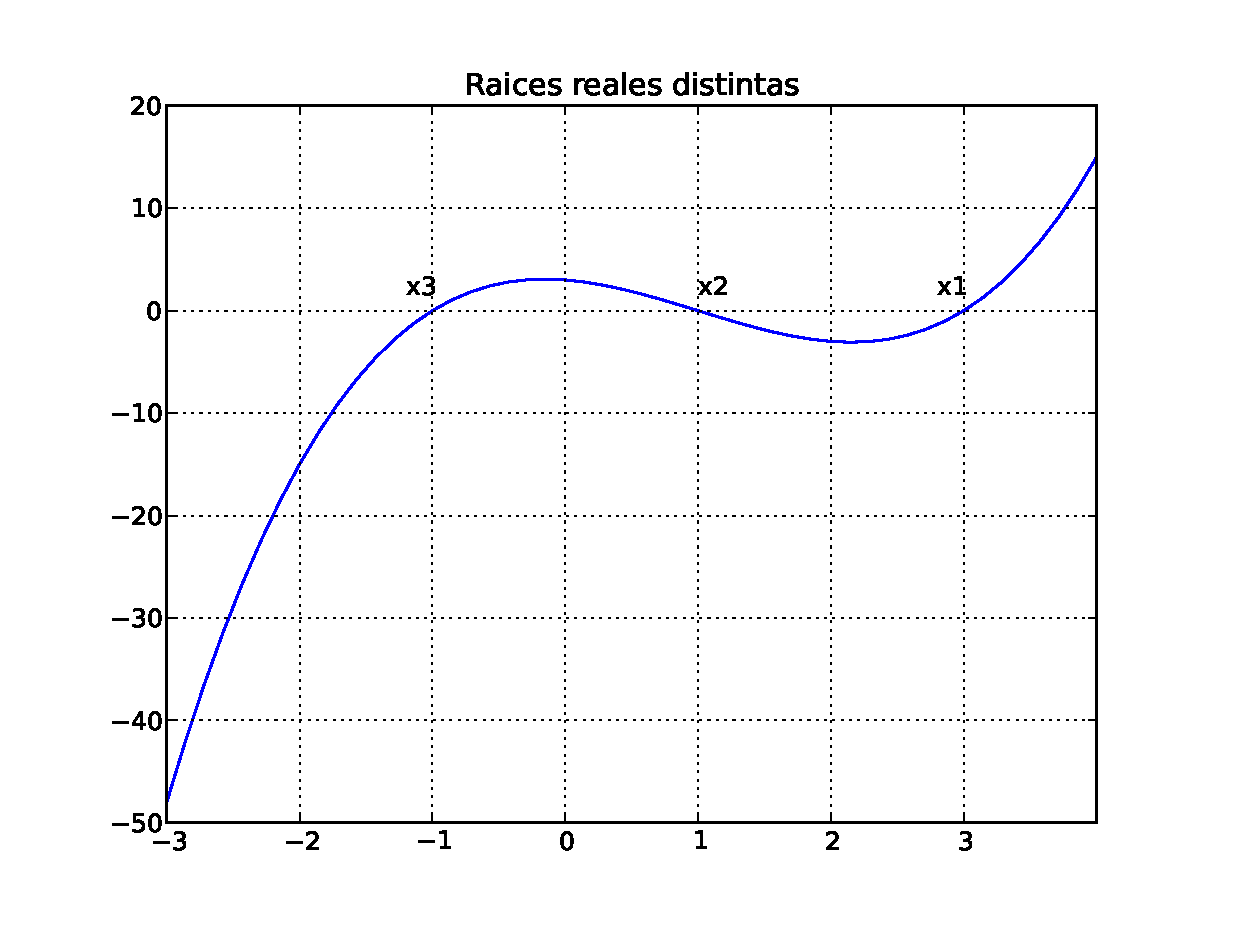
\includegraphics[scale=0.4]{Imagenes/raices01.eps}
	%\vspace{0.5cm}
	\caption{Los valores $x_{i}$ representan las raíces del polinomio.}
\end{figure}
\end{frame}
\begin{frame}[fragile]
% \setbeamerfont{caption}{size=\scriptsize}
% \captionsetup{justification=centering}
\frametitle{Raíz real con multiplicidad 3}
\begin{eqnarray*}
\begin{aligned}
f (x) &=  x^{3} - 6 \: x^{2} + 12 \: x - 8 \\ \pause
&= (x - 2)^{3}
\end{aligned}
\end{eqnarray*}
\pause
Las raíces son:
\begin{align*}
x_{1} &= 2 \hspace{1cm}  x_{2} = 2 \hspace{1cm}  x_{3} = 2
\end{align*}
\end{frame}
\begin{frame}[fragile]
\frametitle{Raíz real con multiplicidad 3}
\begin{figure}
	\centering
	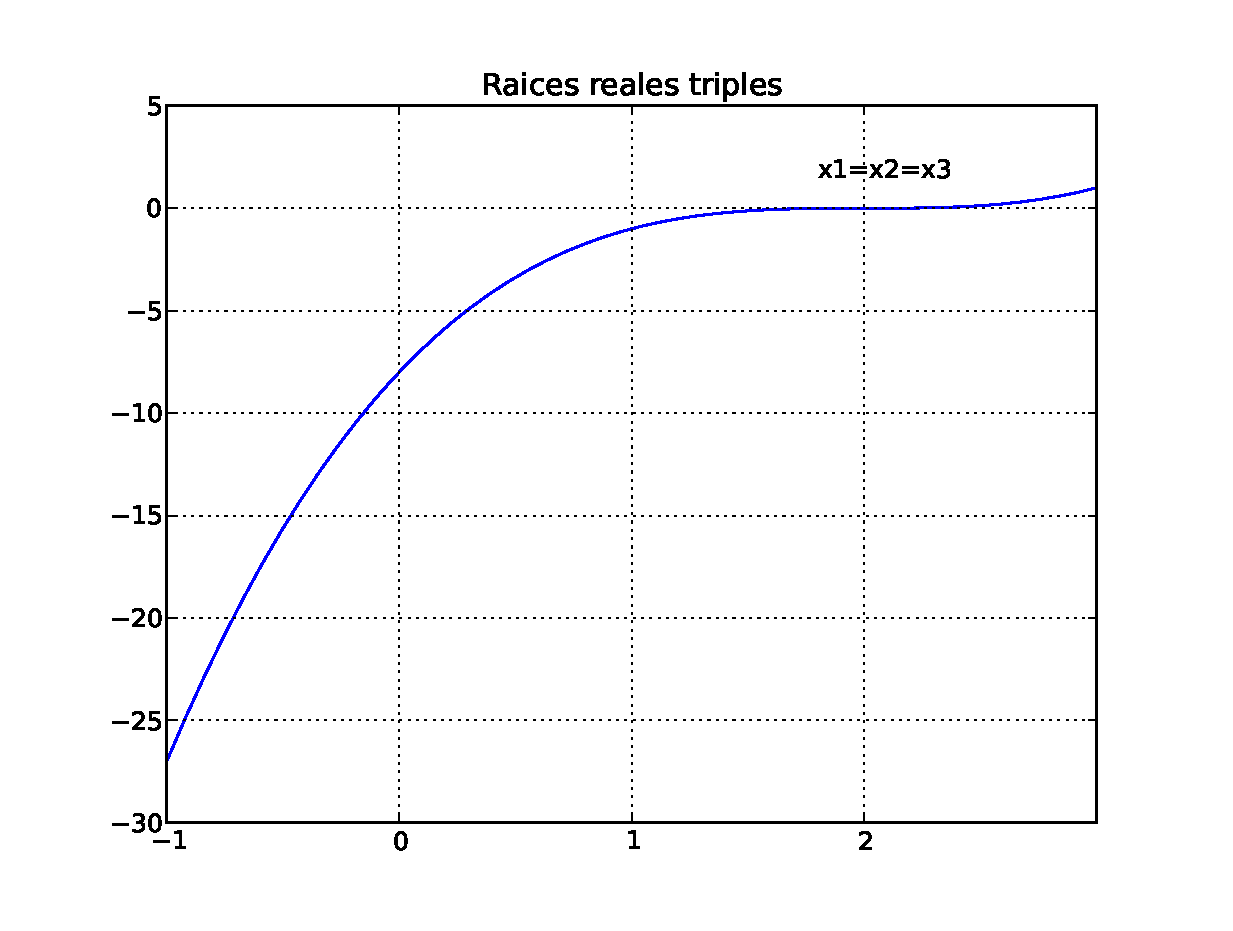
\includegraphics[scale=0.4]{Imagenes/raices02.eps}
	\caption{El valor de las raíces $x_{i}$ coinciden.} 
\end{figure}
\end{frame}
\begin{frame}[fragile]
% \setbeamerfont{caption}{size=\scriptsize}
% \captionsetup{justification=centering}
\frametitle{Raíz real y una raíz real con multiplicidad 2}
\begin{eqnarray*}
\begin{aligned}
f (x) &= x^{3} - 12 \: x + 16 \\ \pause
&= (x + 4)(x - 2)^{2}
\end{aligned}
\end{eqnarray*}
Las raíces son:
\begin{align*}
x_{1} &= -4 \\
x_{2} &= 2 \\
x_{3} &= 2 \\
\end{align*}
\end{frame}
\begin{frame}[fragile]
\frametitle{Raíz real y una raíz real con multiplicidad 2}
\begin{figure}
	\centering
	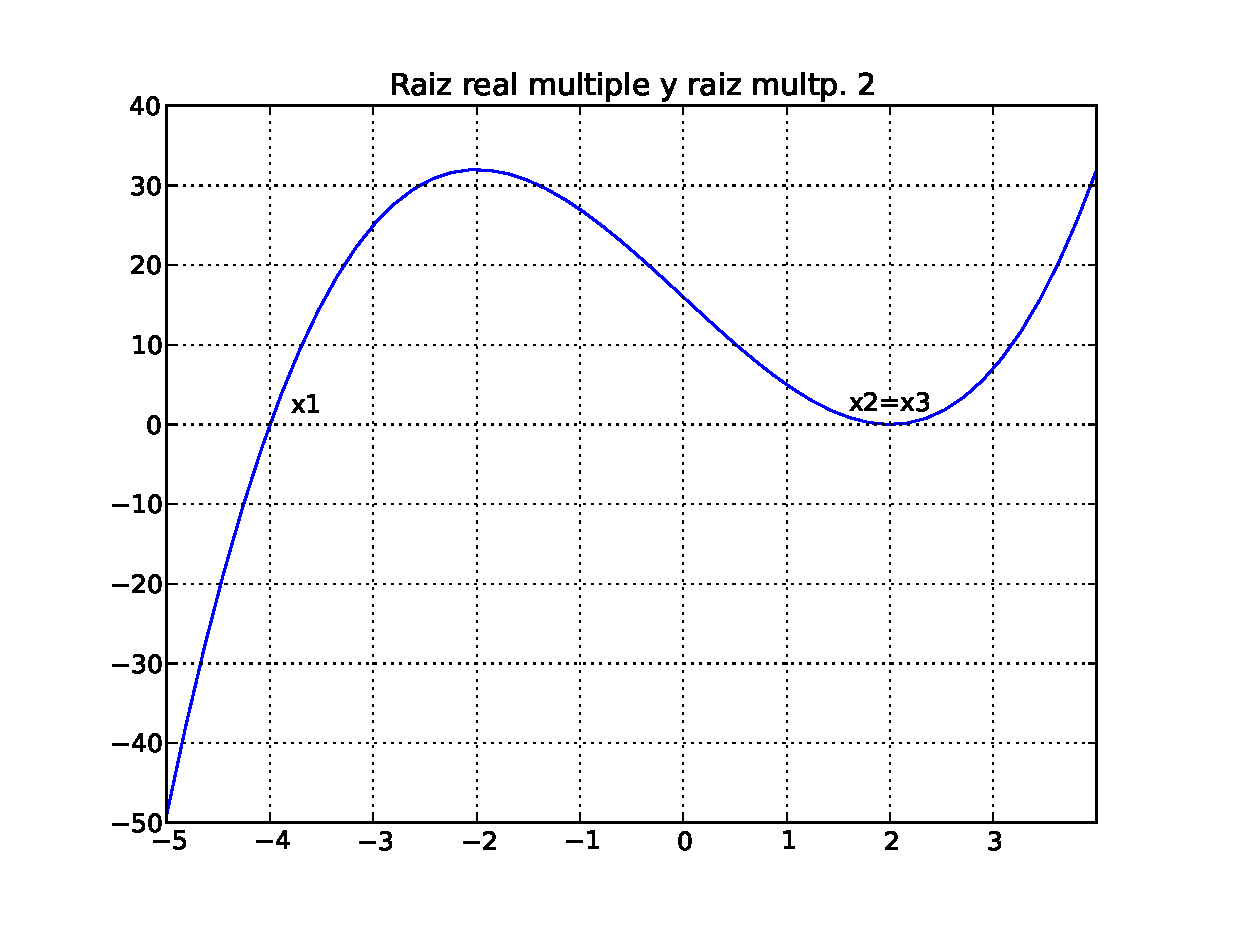
\includegraphics[scale=0.4]{Imagenes/raices03.eps} 
	\caption{Dos valores de las raíces coinciden.}
\end{figure}
\end{frame}
\begin{frame}[fragile]
% \setbeamerfont{caption}{size=\scriptsize}
% \captionsetup{justification=centering}
\frametitle{Raíz real y un par conjugado complejo}
\begin{eqnarray*}
\begin{aligned}
f (x) &= x^{3} - 2 \: x^{2} - 3 \: x + 10  \\  \pause
&= (x + 2) [x - (2 + i)] [x - (2 - i)]
\end{aligned}
\end{eqnarray*}
Las raíces son:
\pause
\begin{align*}
x_{1} &= -2 \hspace{1cm} x_{2} = 2 + i \hspace{1cm} x_{3} = 2 - i
\end{align*}
\end{frame}
\begin{frame}[fragile]
\frametitle{Raíz real y un par conjugado complejo}
\begin{figure}
	\centering
	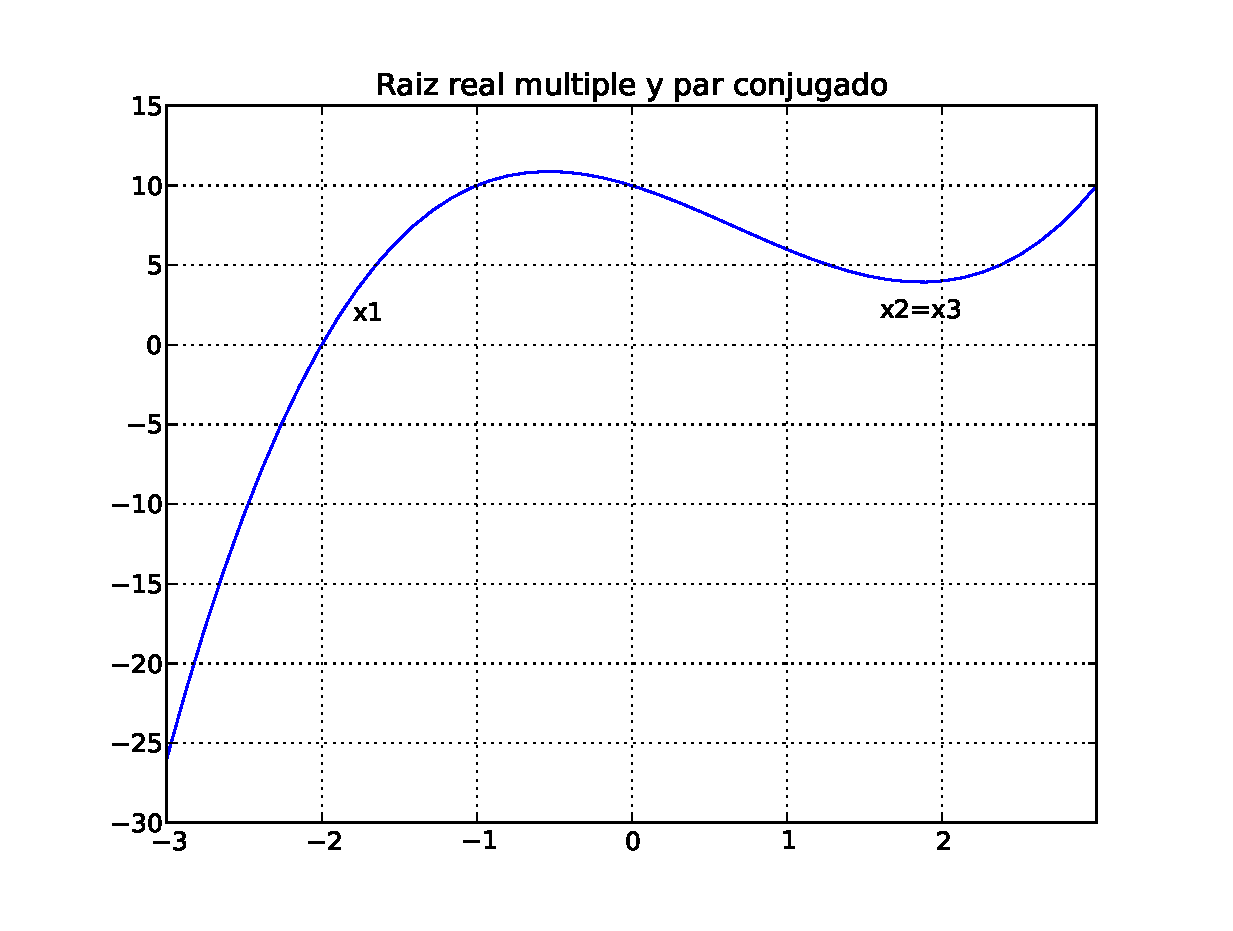
\includegraphics[scale=0.4]{Imagenes/raices04.eps} 
	\caption{Dos valores de las raíces son complejos.}
\end{figure}
\end{frame}

\section{Tipos de funciones}
\frame{\tableofcontents[currentsection, hideothersubsections]}
\subsection{Funciones algebraicas}

\begin{frame}
\frametitle{Funciones algebraicas}
Sea $g = f (x)$ la función expresada como:
\pause
\begin{align*}
f_{n} \: y^{n} + f_{n-1} \: y^{n - 1} + \ldots + f_{1} \: y + f_{0} = 0
\end{align*}
Donde $f_{i}$ es un polinomio de orden $i$ en $x$.
\end{frame}
\begin{frame}
\frametitle{Funciones algebraicas}
Los polinomios son un caso simple de funciones algebraicas que se representan generalmente como:
\begin{align*}
f_{n} (x) = a_{0} + a_{1} \: x + a_{2} \: x^{2}+ \ldots +a_{n} \: x^{n}
\end{align*}
Donde $n$ es el orden del polinomio.
\end{frame}

\subsection{Funciones trascendentales}

\begin{frame}
\frametitle{Funciones trascedentales}
Son aquellas funciones que no son algebraicas. \pause Comprenden a las funciones trigonométricas, exponenciales, logarítmicas, entre otras.
\\
\bigskip
\pause
Ejemplos:
\begin{eqnarray*}
\begin{aligned}
f (x) &= \ln(x^{2} - 1) \\ \pause
g (x) &= e^{-0.2 \: x} \, \sin(3 \: x - 5)
\end{aligned}
\end{eqnarray*}
\end{frame}

\subsection{Calculando las raíces}

\begin{frame}
\frametitle{Encontrar las raíces}
Los métodos numéricos estándar para encontrar raíces pueden clasificarse en dos rubros:
\pause
\setbeamercolor{item projected}{bg=ao,fg=white}
\setbeamertemplate{enumerate items}{%
\usebeamercolor[bg]{item projected}%
\raisebox{1.5pt}{\colorbox{bg}{\color{fg}\footnotesize\insertenumlabel}}%
}
\begin{enumerate}[<+->]
\item La determinación de las raíces reales de ecuaciones algebraicas y trascendentales.
\\
\bigskip
\pause
Las técnicas a emplear en estos casos se diseñaron con el fin de encontrar el valor de una raíz simple de acuerdo con un conocimiento previo de su posición aproximada.
\seti
\end{enumerate}
\end{frame}
\begin{frame}
\frametitle{Encontrar las raíces}
\setbeamercolor{item projected}{bg=ao,fg=white}
\setbeamertemplate{enumerate items}{%
\usebeamercolor[bg]{item projected}%
\raisebox{1.5pt}{\colorbox{bg}{\color{fg}\footnotesize\insertenumlabel}}%
}
\begin{enumerate}[<+->]
\conti    
\item La determinación de todas las raíces reales y complejas de un polinomio, para lo cual los métodos numéricos estén diseñados específicamente para polinomios. 
\\
\bigskip
\pause
Determinan sistemáticamente todas las raíces del polinomio en lugar de hacerlo sólo con una, dada la posición aproximada.
\end{enumerate}
\end{frame}

\section{Método de incrementos sucesivos}
\frame{\tableofcontents[currentsection, hideothersubsections]}
\subsection{El método de incrementos sucesivos}

\begin{frame}
\frametitle{Método de incrementos sucesivos}
Podemos aproximar mucho mejor las raíces de una función, cuando la graficamos.
\\
\bigskip
\pause
Con una gráfica general de unos cuantos puntos, tendríamos lo necesario para considerar los valores de las raíces.
\end{frame}
\begin{frame}
\frametitle{Método de incrementos sucesivos}
El método de \textcolor{blue-violet}{búsqueda incremental} es una herramienta útil que podemos adoptar en conjunto con otras estrategias de cálculo de raíces.
\\
\bigskip
\pause
Éste método no nos ofrece más que una referencia sobre el intervalo en dónde podría(n) estar la(esas) raíces.
\end{frame}
\begin{frame}
\frametitle{Método de incrementos sucesivos}
La idea básica detrás del método de búsqueda incremental es simple: si $f(x_{1})$ y $f(x_{2})$ tienen signos opuestos, entonces hay al menos una raíz en el intervalo $(x_{1}, x_{2})$.
\end{frame}
\begin{frame}[fragile]
\frametitle{Caso en donde es posible encontrar la raíz}
\begin{figure}
	\centering
	\includestandalone{Figuras/figura_raices_01}
	\caption{Los puntos de la función evaluada en los extremos tienen signos contrarios.}
\end{figure}
\end{frame}
\begin{frame}[fragile]
\frametitle{Caso en donde no es posible encontrar la raíz}
\begin{figure}
	\centering
	\includestandalone{Figuras/figura_raices_02}
	\caption{Los puntos de la función evaluada en los extremos tienen el mismo signo.}
\end{figure}
\end{frame}
\begin{frame}
\frametitle{Cuando hay una raíz}
Si el intervalo es lo suficientemente pequeño, es probable que contenga una sola raíz.
\\
\bigskip
\pause
Así, los ceros de $f (x)$ puede ser detectados mediante la evaluación de la función en  intervalos $\Delta \: x$ y mirando cuando se presente un cambio de signo en la función.
\end{frame}
\begin{frame}
\frametitle{Consideraciones con el método}
Hay varios problemas con el método de incrementos sucesivos:
\setbeamercolor{item projected}{bg=bubblegum,fg=burntumber}
\setbeamertemplate{enumerate items}{%
\usebeamercolor[bg]{item projected}%
\raisebox{1.5pt}{\colorbox{bg}{\color{fg}\footnotesize\insertenumlabel}}%
}
\begin{enumerate}[<+->]
\item Es posible perder dos raíces muy próximas entre sí, si el incremento de búsqueda $\Delta \: x$ es mayor que la separación de las raíces.
\item Una raíz doble (dos raíces que coinciden) no será detectada.
\seti
\end{enumerate}
\end{frame}
\begin{frame}
\frametitle{Consideraciones con el método}
\setbeamercolor{item projected}{bg=bubblegum,fg=burntumber}
\setbeamertemplate{enumerate items}{%
\usebeamercolor[bg]{item projected}%
\raisebox{1.5pt}{\colorbox{bg}{\color{fg}\footnotesize\insertenumlabel}}%
}
\begin{enumerate}[<+->]
\conti
\item Algunas singularidades de $f (x)$ se puede confundir con raíces. Por ejemplo, $f (x) = \tan x$. Tiene cambios de signo en $x = \pm 1/2 n \, \pi$ con $n = 1, 3, 5,\ldots$
\end{enumerate}
\end{frame}
\begin{frame}
\frametitle{Casos en donde no hay una raíz}
\begin{figure}
	\centering
	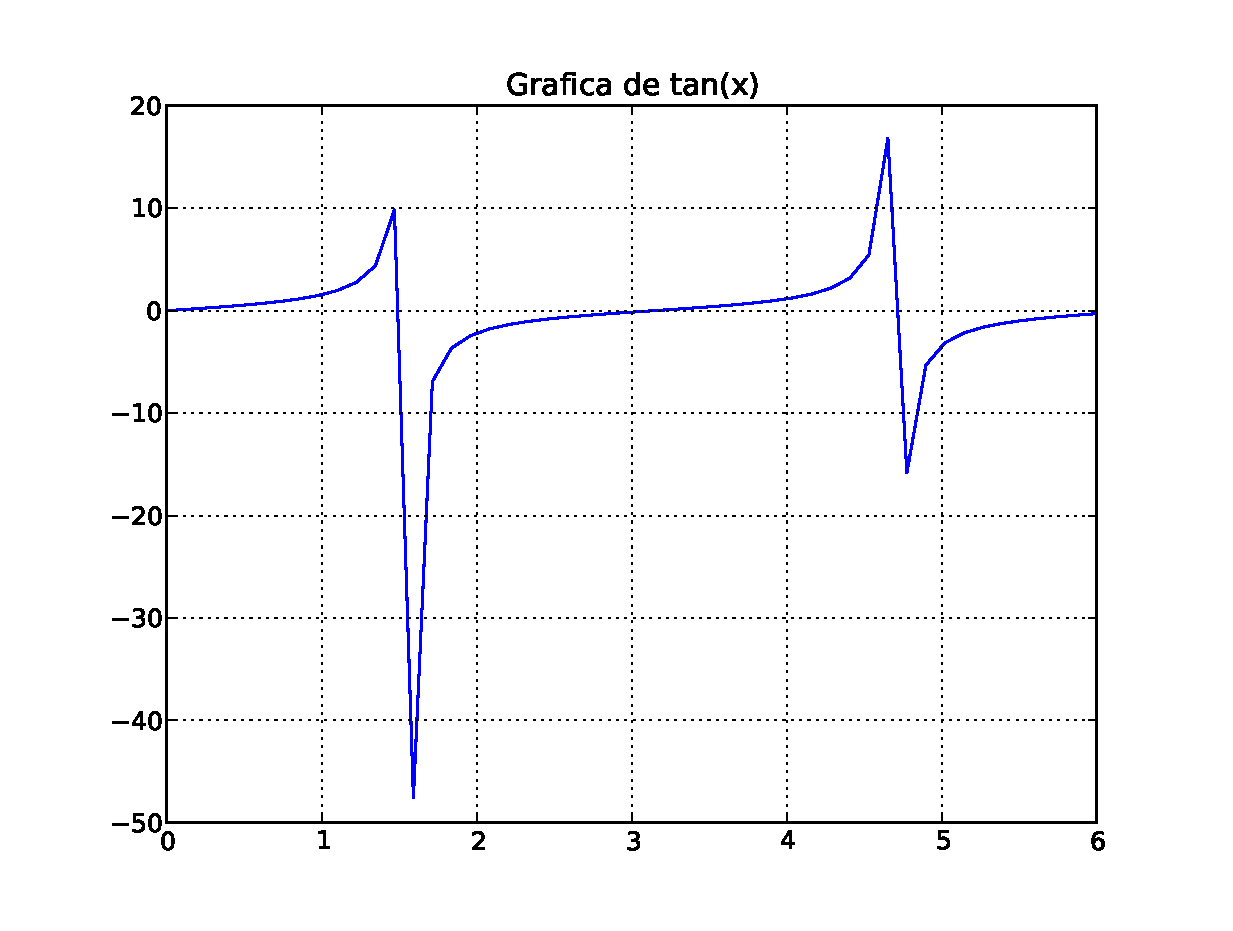
\includegraphics[scale=0.4]{Imagenes/raices05.eps}
	\caption{Estos puntos no son ceros verdaderos, ya que la función no cruza el eje $x$.}
\end{figure}
\end{frame}

\subsection{Código python}

\begin{frame}
\frametitle{Código Método de incrementos sucesivos}
El código busca un cero de la función $f$ que proporciona el usuario en el intervalo
$(a, b)$ en incrementos de $dx$.
\\
\bigskip
\pause
Se devuelve el intervalo $(x_{1}, x_{2})$ donde se encuentra la raíz, si la búsqueda
se ha realizado correctamente; se devuelve $x_{1} = x_{2} = \mathsf{None}$ cuando no se encontraron raíces.
\end{frame}
\begin{frame}
\frametitle{Código Método de incrementos sucesivos}
Luego de que se encontró la primera raíz, (la más cercana al punto $a$), se puede llamar de nuevo al procedimiento, sustitiyendo $x_{2}$ con el fin de encontrar la siguiente raíz. 
\\
\bigskip
\pause
Esto se puede repetir siempre y cuando se detecta una raíz.
\end{frame}
\begin{frame}[fragile]
\frametitle{Función \azulfuerte{\texttt{buscaraiz}}}
\begin{lstlisting}[caption=Función buscaraiz para encontrar un intervalo que contiene una raíz]
def buscaraiz(f, a, b, dx):
    x1 = a; f1 = f(a)
    x2 = a + dx; f2 = f(x2)
    while f1 * f2 > 0.0:
        if x1 >= b: return None
        x1 = x2; f1 = f2
        x2 = x1 + dx; f2 = f(x2)
    else:
        return x1, x2
\end{lstlisting}
\end{frame}

\subsection{Ejercicio}

\begin{frame}
\frametitle{Ejemplo para encontrar una raíz}
Usa el método de incrementos sucesivos con espaciamientos de $\Delta x = 0.2$, para estimar la raíz con el valor positivo más pequeño de la función:
\pause
\begin{align*}
f (x) = x^{3} - 10 x^{2} + 5
\end{align*}
\end{frame}
\begin{frame}
\frametitle{¿Cómo resolver el problema?}
Como el ejercicio pide que se localice la raíz positiva más pequeña, habrá que tener una idea sobre el comportamiento de la función.
\\
\bigskip
\pause
Para ello, graficamos en un intervalo inicial, considera que hay potencias al cubo.
\end{frame}
\begin{frame}
\frametitle{Gráfica inicial de la función}
\begin{figure}
	\centering
	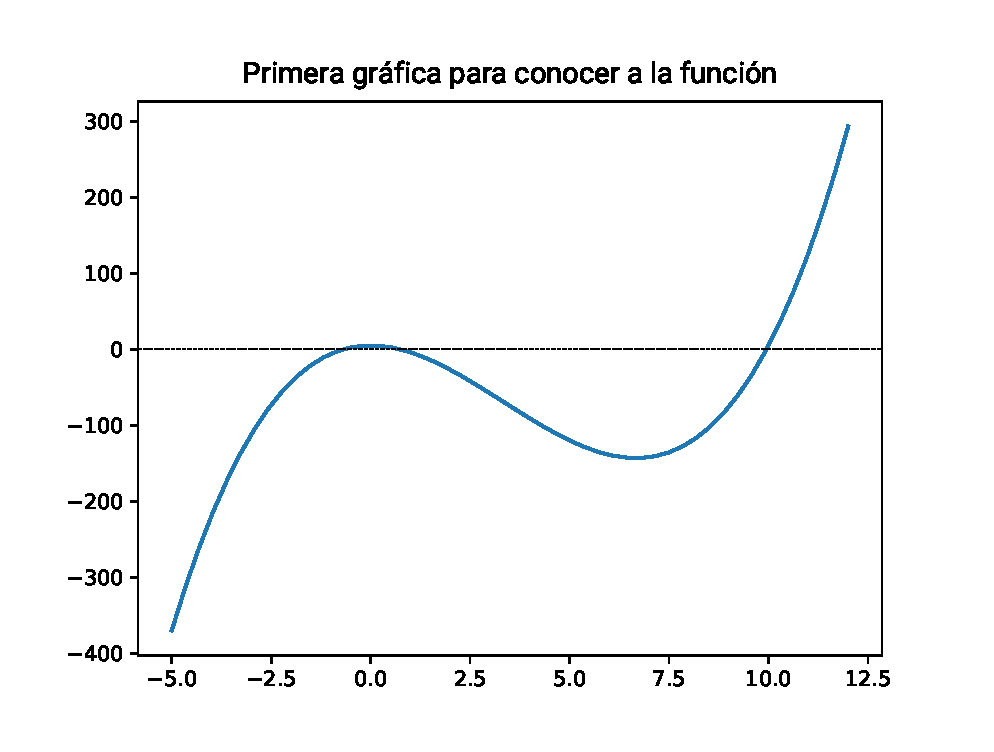
\includegraphics[scale=0.5]{Imagenes/aprox_sucesivas_01.eps}
	\caption{De la gráfica vemos que hay tres raíces, que cruzan el eje $y = 0$.} 
\end{figure}
\end{frame}
\begin{frame}
\frametitle{Una mejora en la gráfica}
\begin{figure}
    \centering
    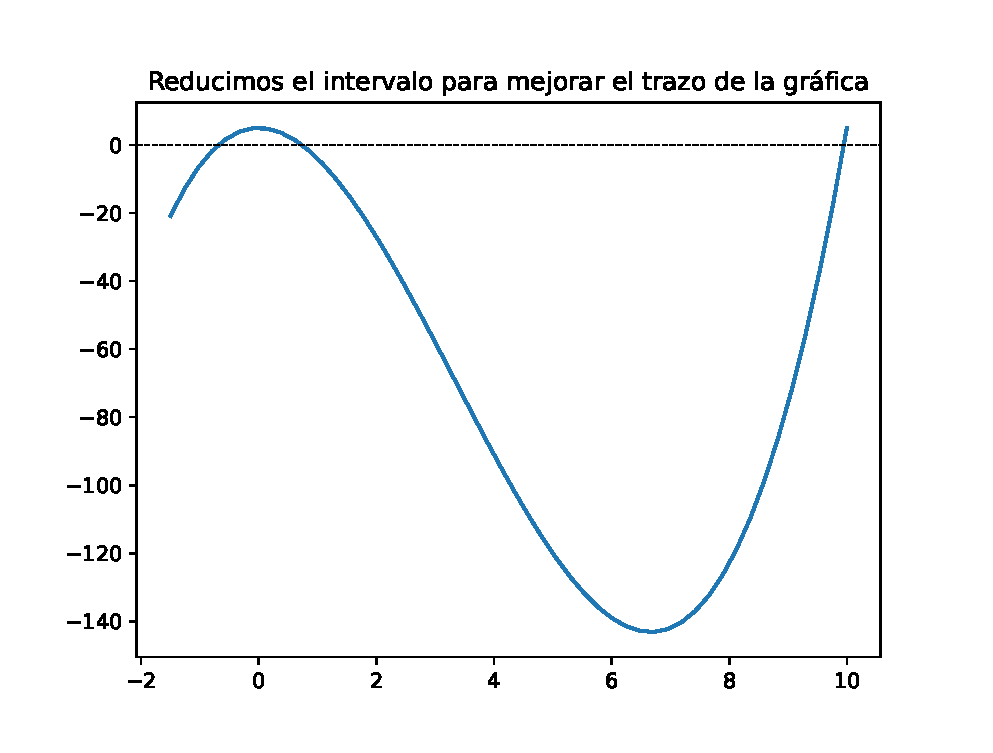
\includegraphics[scale=0.5]{Imagenes/aprox_sucesivas_01b.eps}
    \caption{Las raíces ya se muestran mejor.} 
\end{figure}
\end{frame}
\begin{frame}
\frametitle{Acotando el problema}
Como se nos pide el valor de la raíz positiva más pequeña, descartamos las raíz negativa y la otra raíz positiva.
\\
\bigskip
\pause
En la siguiente gráfica se reduce el intervalo sobre el eje $x$ para tener una mejor vista.
\end{frame}
\begin{frame}
\frametitle{El intervalo de la gráfica se ha acotado}
\begin{figure}
	\centering
	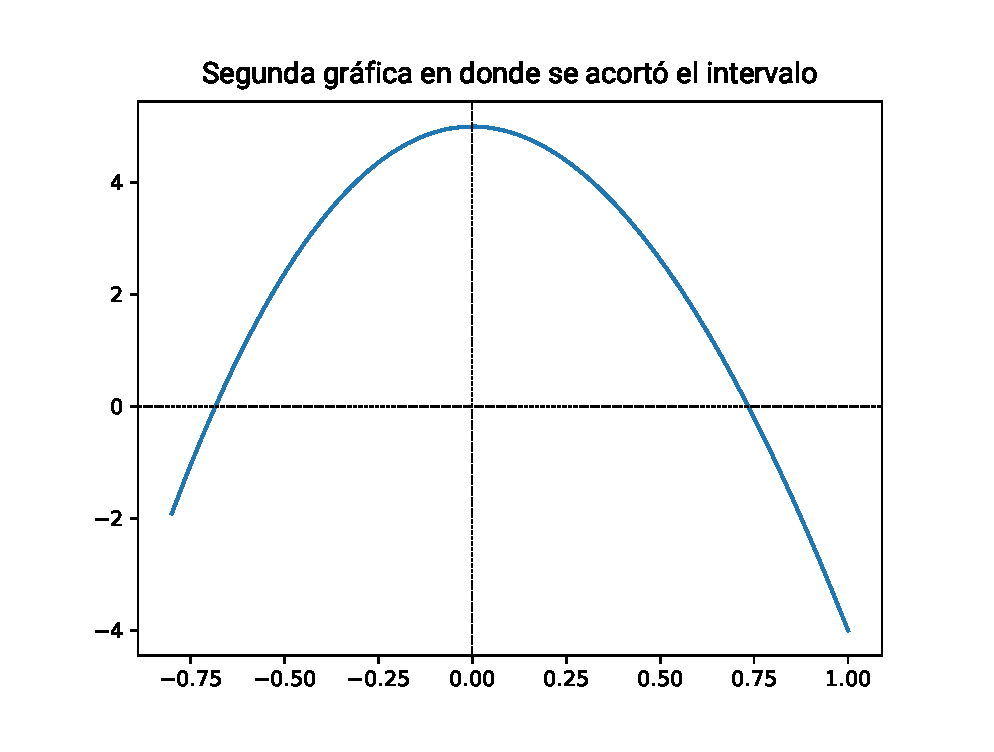
\includegraphics[scale=0.5]{Imagenes/aprox_sucesivas_02.eps}
\end{figure}
\end{frame}
\begin{frame}
\frametitle{Ajustando visualmente}
Se aprecia mucho mejor al reducir el intervalo en la gráfica.
\\
\bigskip
\pause
Nos falta aún calcular el intervalo donde está la raíz positiva más pequeña, para ello usaremos el siguiente código.
\end{frame}
\begin{frame}[fragile]
\frametitle{Ahora con \python}
\begin{lstlisting}[caption=Solución al ejercicio]
def f(x): return x**3 - 10 * x**2 + 5.

a, b, dx = (0.0, 1.5, 0.2)

x1, x2 = buscaraiz(f, a, b, dx)
print('La raiz esta en el intervalo: ({0:1.3f}, {1:2.3f})'.format(x1, x2))
\end{lstlisting}
\end{frame}
\begin{frame}
\frametitle{El intervalo de trabajo}
\begin{figure}
	\centering
	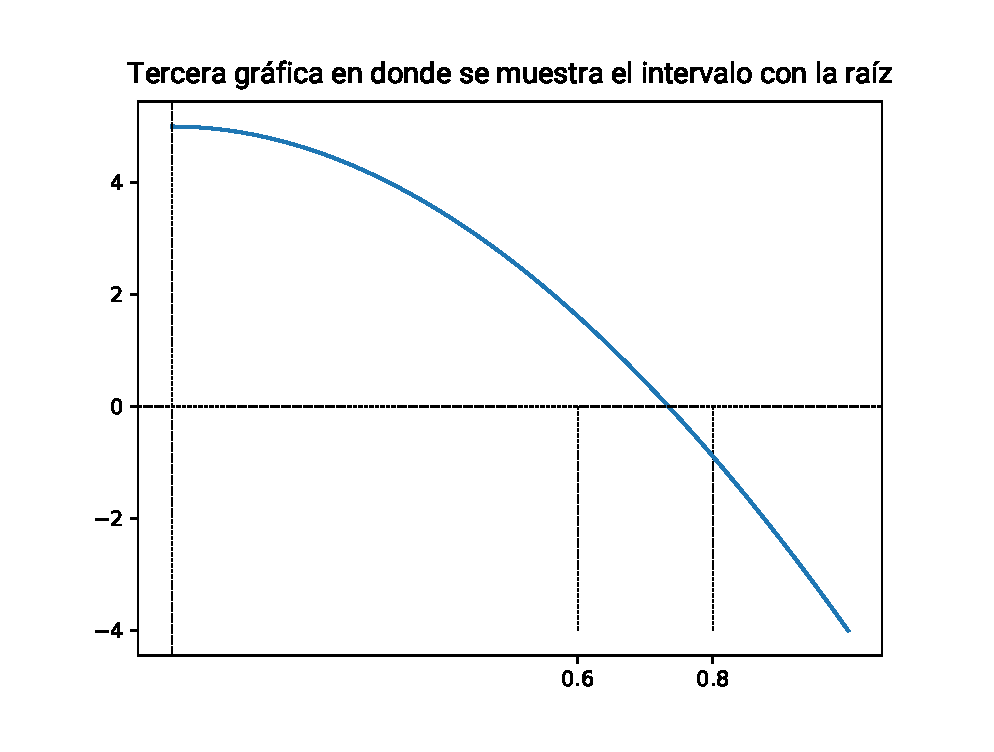
\includegraphics[scale=0.5]{Imagenes/aprox_sucesivas_03.eps}
\end{figure}
\end{frame}
\begin{frame}
\frametitle{Intervalo obtenido}
El código de \python{} devuelve el intervalo de interés, es decir, donde se encuentra una raíz de la función.
\\
\bigskip
\pause
El siguiente paso es definir alguna técnica para calcular el valor de la raíz.
\end{frame}

\section{Métodos para el cálculo de raíces}
\frame{\tableofcontents[currentsection, hideothersubsections]}
\subsection{Método de Bisección}

\begin{frame}
\frametitle{Método de Bisección}
Después de que se ha identificado una raíz $ f(x) = 0$ en el intervalo $(x_{1}, x_{2})$, disponemos de varios métodos para encontrar el valor de la raíz.
\end{frame}
\begin{frame}
\frametitle{Método de Bisección}
El \textcolor{cadmiumgreen}{método de bisección} logra esta tarea: \pause \textcolor{red}{el intervalo se reduce sucesivamente a la mitad  hasta que se vuelve suficientemente pequeño}. 
\end{frame}
\begin{frame}
\frametitle{Método de Bisección}
La técnica de bisección \textit{no es el método más rápido} disponible, pero es el más fiable.
\\
\bigskip
\pause
Una vez que una raíz se ha encontrado en un intervalo, nos podemos acercar a ella.
\end{frame}
\begin{frame}
\frametitle{Funcionamiento del método}
El método de bisección utiliza el mismo principio que el de incrementos sucesivos: \pause si hay una raíz en el intervalo $(x_{1}, x_{2})$, entonces revisa si $f(x_{1}) * f(x_{2}) < 0$.
\end{frame}
\begin{frame}
\frametitle{Funcionamiento del método}
Con el fin de reducir a la mitad el intervalo, se calcula $f (x_{3})$, donde $x_{3} = (x_{1} + x_{2})/2$ es el punto medio del intervalo.
\end{frame}
\begin{frame}
\frametitle{Descripción gráfica del método de bisección}
\setbeamercovered{invisible}
\begin{figure}
	\centering
	\includestandalone{Figuras/biseccion_01}
\end{figure}
\end{frame}
\begin{frame}
\frametitle{Funcionamiento del método}
Si $f (x_{1}) * f (x_{3}) < 0$ entonces la raíz debe estar en $(x_{1}, x_{3})$, \pause entonces reemplazamos del intervalo inicial $x_{2}$ por $x_{3}$, y se repite la división del intervalo.
\setbeamercovered{invisible}
\pause
\begin{figure}
	\centering
	\includestandalone{Figuras/biseccion_02}
\end{figure}
\end{frame}
\begin{frame}
\frametitle{Funcionamiento del método}
De lo contrario, la raíz se encuentra en el intervalo $(x_{3}, x_{2})$, en tal caso, se sustituye $x_{3}$ por $x_{1}$, y se repite la división del intervalo.
\end{frame}
\begin{frame}
\frametitle{¿Hasta cuando se repite la división del intervalo?}
En cualquiera de los casos, el nuevo intervalo $(x_{1}, x_{2})$ es la mitad del tamaño del intervalo original.
\\
\bigskip
\pause
La bisección es repite hasta que el intervalo se ha reducido a un valor $\varepsilon$ pequeño, de modo que:
\begin{align*}
\abs{ x_{2} - x_{1} } \leq \varepsilon
\end{align*}
\end{frame}
\begin{frame}
\frametitle{Estimar el número de divisiones del intervalo}
Es fácil calcular el número de bisecciones necesarias para alcanzar el valor de $\varepsilon$.
\\
\bigskip
\pause
El intervalo inicial $\Delta \: x$, se reduce a $\Delta \: x /2$ en la primera bisección, $\Delta \: x /2^{2}$ en la segunda, luego de $n$ bisecciones, $\Delta \: x /2^{n}$.
\end{frame}
\begin{frame}
\frametitle{Estimar el número de divisiones del intervalo}
Haciendo $\Delta \: x /2^{n} = \varepsilon$, resolvemos para $n$:
\pause
\begin{align*}
n = \dfrac{\ln( \abs{ \Delta x } / \varepsilon)}{\ln 2}
\end{align*}
\end{frame}

\subsection{\texttt{moduloRaices}}

\begin{frame}
\frametitle{Usando un módulo para los métodos}
Continuaremos trabajando con un módulo en donde dejaremos las funciones de los métodos para estimar el valor de la raíces.
\\
\bigskip
\pause
El nombre del módulo será: \funcionazul{moduloRaices}.
\end{frame}
\begin{frame}
\frametitle{Agregando otras técnicas}
Las siguientes técnicas que trabajemos en el tema deberán de incluirse en el módulo \funcionazul{moduloRaices}.
\\
\bigskip
\pause
De tal manera que en la entrega de ejercicios y Examen Tarea, se debe de hacer referencia e incluir ese módulo.
\end{frame}

\subsection{Bisección en python}

\begin{frame}[allowframebreaks, fragile]
\frametitle{Función el método de bisección}
\begin{lstlisting}[caption=Método de bisección con \python]
def biseccion(f, x1, x2, switch = 1, tol = 1.0e-9):
    f1 = f(x1)
    if f1 == 0.0: return x1
    
    f2 = f(x2)
    if f2 == 0.0: return x2
    
    if sign(f1) == sign(f2):
        print('La raiz no esta en el intervalo')

    n = int(math.ceil(math.log(abs(x2 - x1)/tol)/math.log(2.0)))
    
    for i in range(n):
        x3 = 0.5 * (x1 + x2); f3 = f(x3)
        if (switch == 1) and (abs(f3) > abs(f1)) \
                    and (abs(f3) > abs(f2)):
                        
            return None
        
        if f3 == 0.0: return x3

        if sign(f2) != sign(f3): x1 = x3; f1 = f3
        else: x2 = x3; f2 = f3
    
    return (x1 + x2)/2.0
\end{lstlisting}
\end{frame}
\begin{frame}
\frametitle{El argumento \texttt{switch}}
Al establecer el valor del argumento \texttt{switch} $=1$, forzamos la rutina para verificar si la magnitud de $f (x)$ disminuye con cada intervalo
a la mitad.
\end{frame}
\begin{frame}
\frametitle{El argumento \texttt{switch}}
Si no lo hace, algo puede estar mal: \pause probablemente la \enquote{raíz}, no es una raíz en absoluto, pero es un polo.
\\
\bigskip
\pause
En ese caso, se devuelve \texttt{raíz = None}. Porque esta característica no siempre es deseable, el valor predeterminado es \texttt{switch} $= 0$.
\end{frame}
\begin{frame}[fragile]
\frametitle{¿Qué hace la función \azulfuerte{\texttt{ceil}}?}
La función \funcionazul{ceil} devuelve el menor entero mayor o igual a $x$.
\\
\medskip
\pause
Ejemplos:\\
\medskip
\verb|>>>ceil(1.1) # 2.0| \\ \pause
\verb|>>>ceil(1.6) # 2.0| \\ \pause
\verb|>>>ceil(-1.1) # -1.0| \\ \pause
\verb|>>>ceil(-1.6) # -1.0|
\end{frame}

\subsection{Ejercicio con bisección}

\begin{frame}[fragile]
\frametitle{Ejercicio con bisección}
Calcular la raíz de:
\begin{align*}
x^{3} - 10 \; x^{2} + 5 = 0
\end{align*}
que se encuentra en el intervalo $(0, 1)$, con una precisión de 4 dígitos. \pause ¿Cuántas evaluaciones se requieren para encontrar la raíz?
\end{frame}
\begin{frame}[fragile]
\frametitle{Ejercicio con bisección}
Como primer punto, generamos una gráfica para tener una idea del comportamiento de la función:
\pause
\begin{figure}
	\centering
	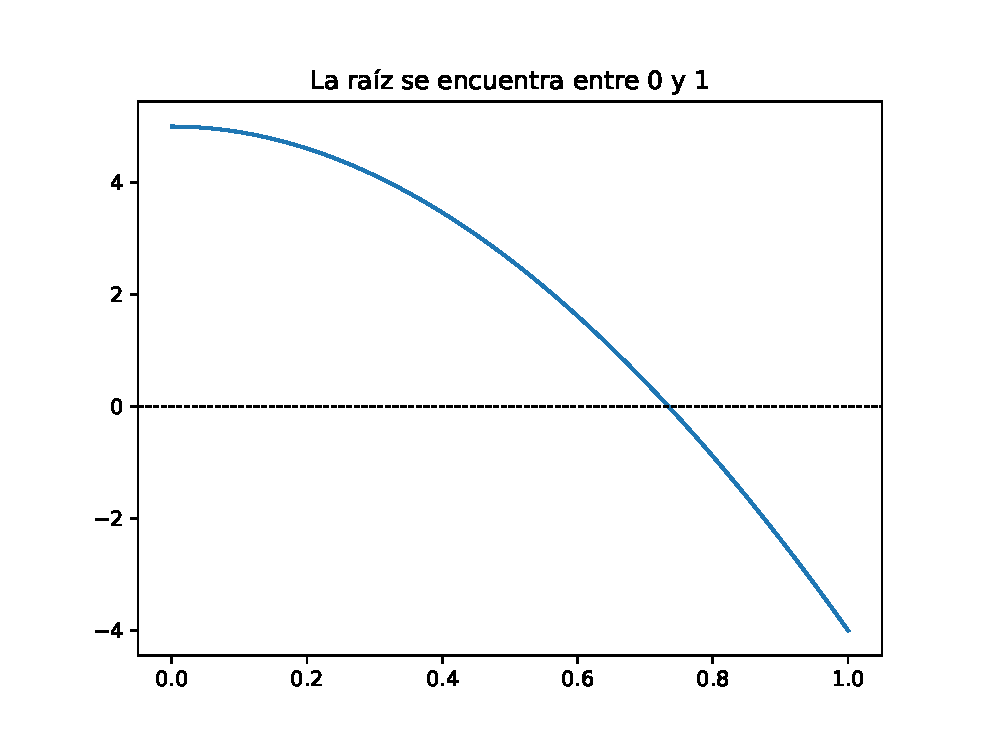
\includegraphics[scale=0.455]{Imagenes/Ejercicio_4_2_Libro.eps}
\end{figure}
\end{frame}
\begin{frame}[allowframebreaks, fragile]
\frametitle{Solución}
\begin{lstlisting}[caption=Solución al ejercicio]
from moduloRaices import biseccion

def f(x): return x**3 - 10.0*x**2 + 5.0

a = 0.
b = 1.
raiz = biseccion(f, a, b, tol = 1.0e-4)

print('La raiz en el intervalo ({0:}, {1:}) es: {2:1.4f}'.format(a, b, raiz))
\end{lstlisting}
\end{frame}
\begin{frame}[fragile]
\frametitle{Solución gráfica}
Una vez calculada la raíz, podemos presentarla en la gráfica
\begin{figure}
	\centering
	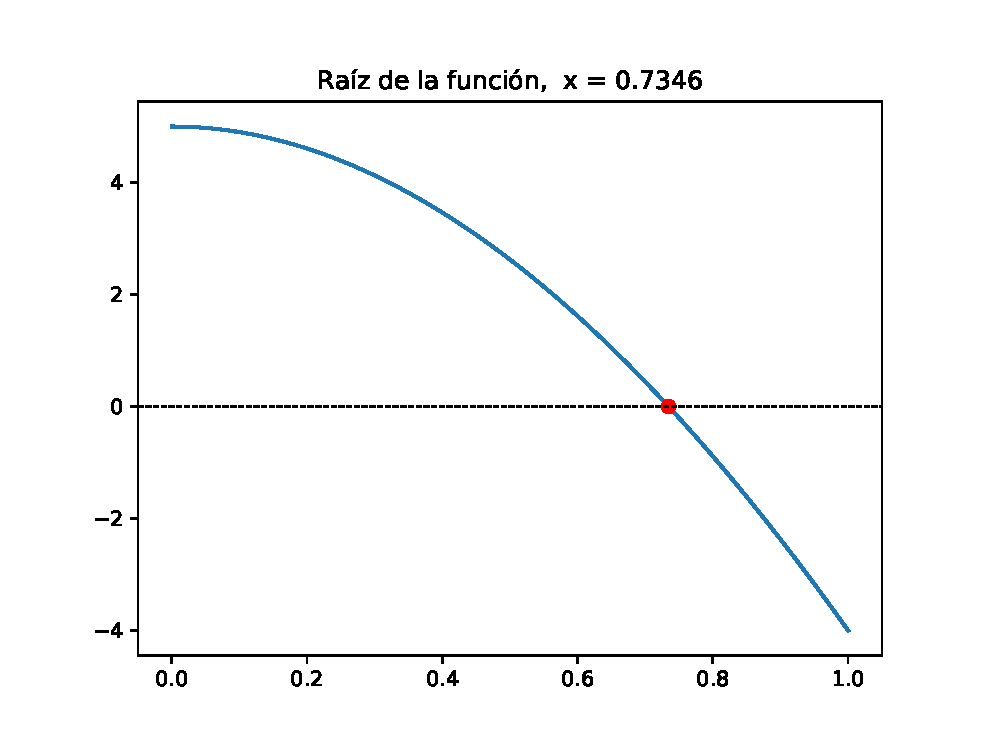
\includegraphics[scale=0.5]{Imagenes/Ejercicio_4_2_02_Libro.eps}
\end{figure}
\end{frame}

\subsection{Ejercicios a cuenta}

\begin{frame}
\frametitle{Ejercicios}
Implementa el método de bisección para calcular el(los) intervalo(s) y la(s) raíz(ces) de:
\pause
\setbeamercolor{item projected}{bg=black,fg=white}
\setbeamertemplate{enumerate items}{%
\usebeamercolor[bg]{item projected}%
\raisebox{1.5pt}{\colorbox{bg}{\color{fg}\footnotesize\insertenumlabel}}%
}
\begin{enumerate}[<+->]
\item $f (x) = x^{3} - 10 \, x^{2} + 5$
\item $g (x) = x - \tan(x) \hspace{1cm} 0 \leq x \leq 20$
\end{enumerate}
Con una tolerancia de $\num{d-9}$.
\end{frame}
\begin{frame}
\frametitle{Consideraciones previas}
Toma en cuenta que $\tan(x)$ es singular y cambia de signo en $x = \pi/2, 3\pi/2,\ldots$. Para no confundir estos puntos para las raíces, hacemos \texttt{switch}= 1.
\\
\medskip
\pause
La proximidad de las raíces a las singularidades es otro problema potencial que puede ser prevenido mediante el uso de $\Delta x$ pequeña, usa $x = 0.01$.
\end{frame}
\begin{frame}
\frametitle{Graficas de las funciones y sus raíces}
\begin{figure}
	\centering
	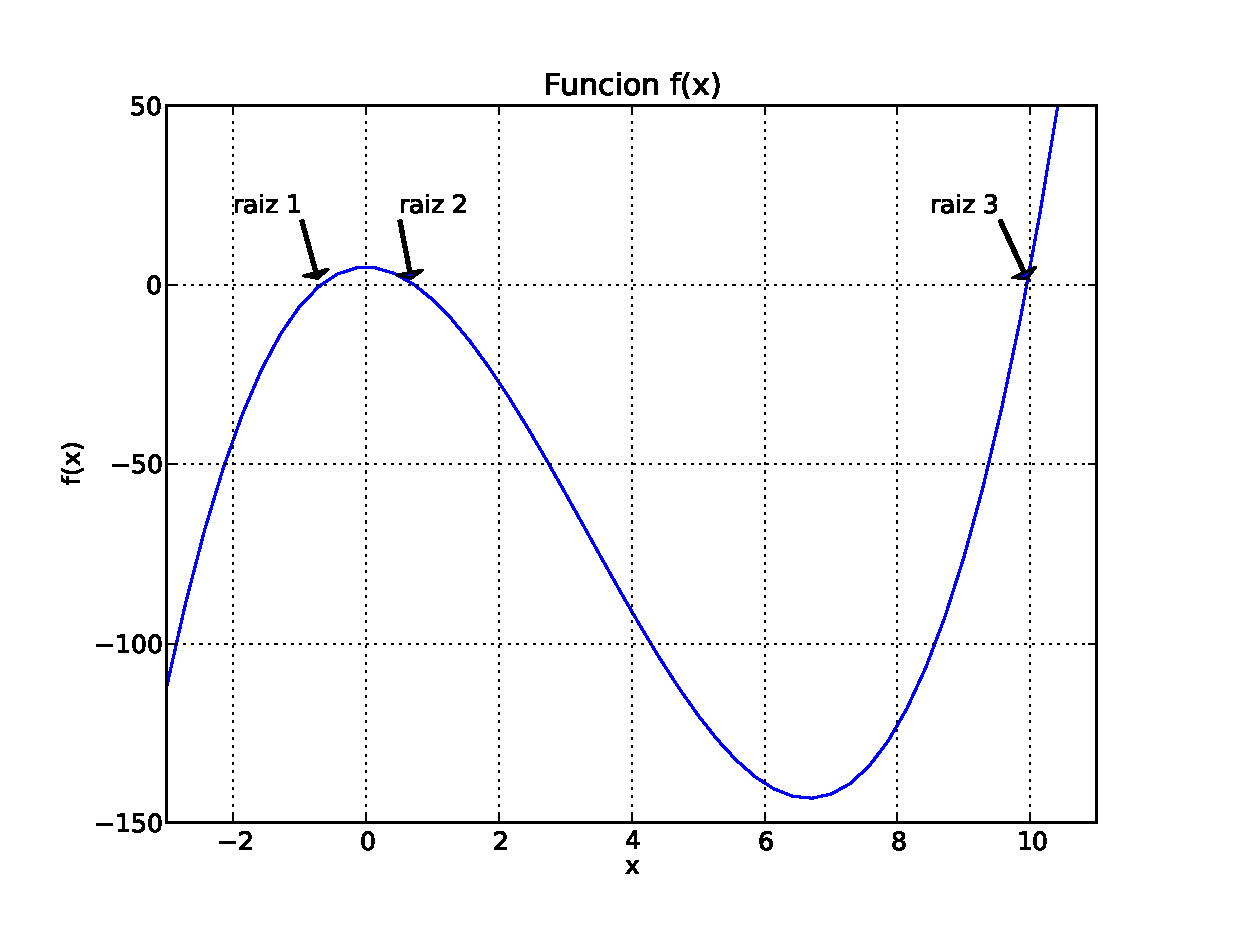
\includegraphics[scale=0.4]{Imagenes/ejercicio1_Biseccion.eps}<1>
	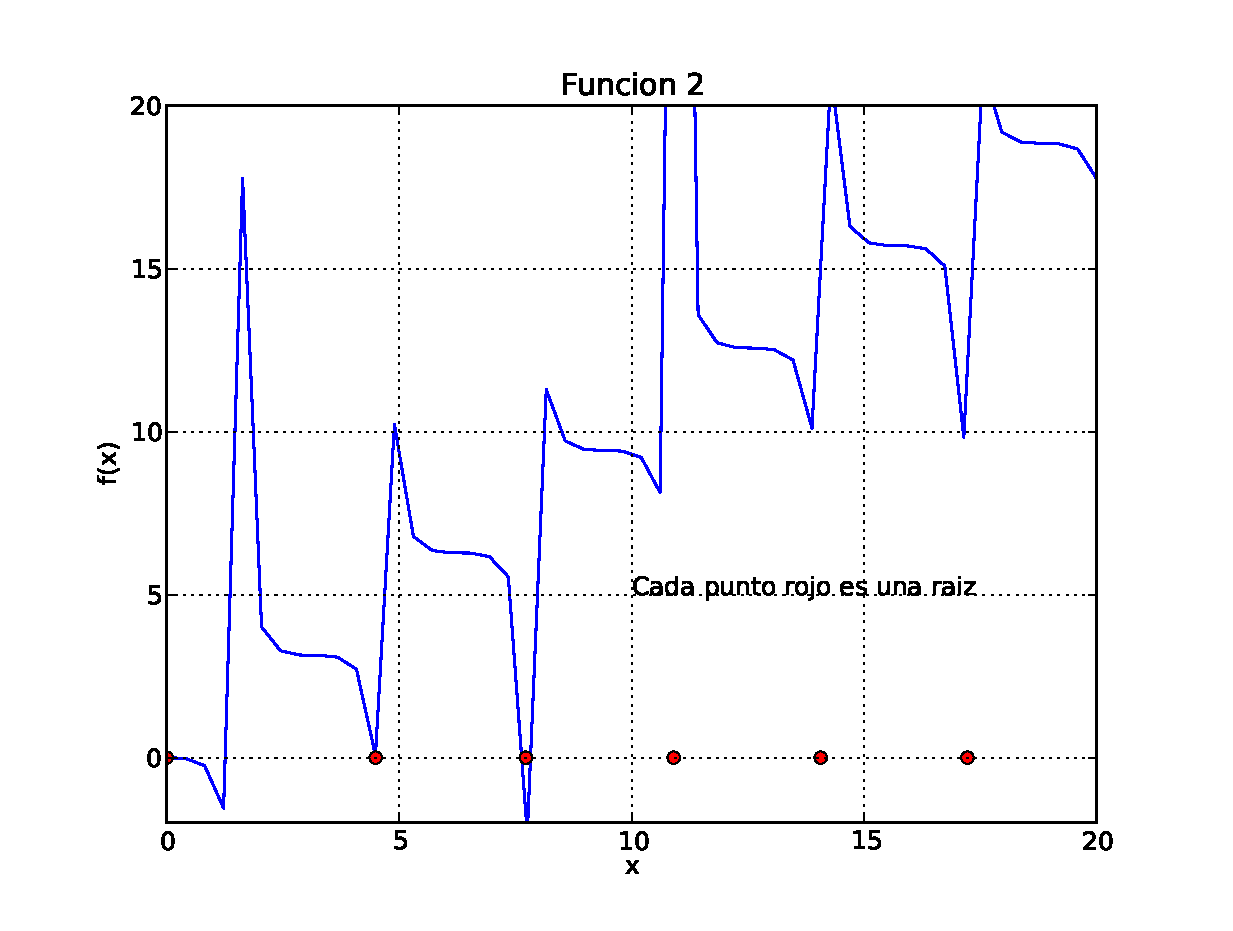
\includegraphics[scale=0.4]{Imagenes/ejercicio2_Biseccion.eps}<2>
\end{figure}
\end{frame}
% % \begin{frame}
% % \frametitle{Estrategia de solución}
% % Para integrar los elementos que hemos visto:
% % \begin{enumerate}
% % \item Recuperamos el algoritmo que nos identifica en qué intervalo se encuentra una raíz.
% % \item Aplicamos el algoritmo del método de bisección.
% % \item Usamos un ciclo que nos revise en el dominio que se nos proporciona, si existe más de una raíz.
% % \end{enumerate}
% % \end{frame}
% % \begin{frame}[fragile]
% % \begin{lstlisting}
% % def f(x): return x**3-10*x**2+5

% % a,b,dx = (-2.0,11.0,0.02)
	
% % print 'Intervalo (x1,x2)   raiz'
% % while 1:
% %     try:
% %         x1, x2 = buscaraiz(f,a,b,dx)
% %     except Exception, e:
% %         print e; break
% %     if x1 != None:
% %         a = x2
% %         root = bisect(f,x1,x2,0)
% %         if raiz != None: print '(%2.4f, %2.4f) %2.8f' %(x1, x2, raiz)
% % \end{lstlisting}
% % \end{frame}
% % \begin{frame}[fragile]
% % \begin{lstlisting}
% %     else:
% %         print '\nHecho'
% %         break
% % \end{lstlisting}
% % \end{frame}
\end{document}